\chapter{Union-Find} 

V~tejto sekcií popíšeme aké operácie Union-Find podporuje, aké sú možnosti využitia tejto dátovej štruktúry, vysvetlíme si ako sme v~rámci tejto práce reprezentovali štruktúru, ako sa operácie tejto štruktúry implementujú a~aké sú možnosti ich optimalizácie.

Pre potreby vysvetlenia akou dátovou štruktúrou Union-Find je a pre vysvetlenie reprezentácie tejto štuktúry je potrebné následujúce názvoslovie:
\begin{itemize}
    \item nezávislé (disjunktné) množiny -- dve množiny nazveme nazávislými práve vtedy, keď ich prienik tvorí prázdnu množinu,
    \item \textbf{grafové názvoslovie...}
\end{itemize}

% TODO:
    % doplň z teórie grafov a pridaj citácie
    % graf, strom, zakorenený strom, cesta, koreň, súvislosť, slučka, stok

\section{Čo to je Union-Find?} \label{union-find_uvod}

Union-Find je dátová štruktúra zložená z~kolekcie nezávislých množín, kde každá množina je identifikovaná jednoznačným identifikátorom. Často je možné sa s~touto dátovou štruktúrou stretnúť aj pod názvom \emph{Merge-Find} alebo \emph{Disjoint Set}.

\begin{figure}[H]
    \centering
    \captionsetup{justification=centering}
    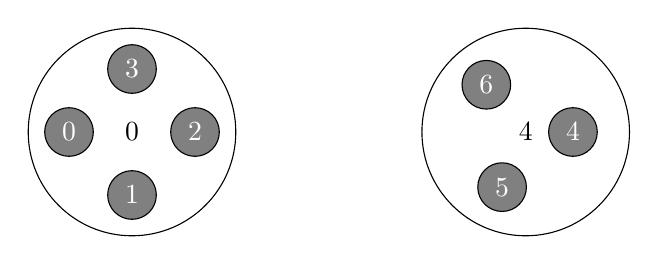
\begin{tikzpicture}
        \tikzset{set/.style = {draw,circle,minimum size=7.5em}}
        \tikzset{element/.style = {draw,circle,fill=gray,text=white}}
        
        \node[set] (0) at (0,0) {0};
        \node[set] (4) at (5,0) {4};

        \node[element] (0) at (-0.8,0) {0};
        \node[element] (1) at (0,-0.8) {1};
        \node[element] (2) at (0.8,0) {2};
        \node[element] (3) at (0,0.8) {3};

        \node[element] (4) at (5.6,0) {4};
        \node[element] (5) at (4.7,-0.7) {5};
        \node[element] (6) at (4.5,0.6) {6};
    \end{tikzpicture}
    \caption{Vennove diagramy reprezentujúce 2 disjunktné množiny s~identifikátormi 1 a 2}
    \label{fig:venn}
\end{figure}

Union-Find podporuje následujúce 3 operácie:

\newpage

\begin{itemize}
    \item pridanie prvku,
    \begin{itemize}
        \item tento novo vložený prvok reprezentuje novú množinu obsahujúcu iba tento prvok,
        \item ako napovedá jeden z~názvov tejto dátovej štruktúry (\emph{Disjoint Set}, v~preklade \emph{disjunktna množina}), štruktúra \textbf{neumožňuje} vkládanie prvkov, ktoré sa už v~niektorej z~množín nachádzajú,
    \end{itemize}
    \item zjednotenie množín
    \begin{itemize}
        \item umožňuje tvorbu množiny obsahujúcej všetky prvky pôvodných 2 množín (a~zánik pôvodných 2 množín),
    \end{itemize}
    \item identifikácia množiny, do ktorej prvok patrí,
    \begin{itemize}
        \item táto operácia umožňuje získať identifikátor množiny, do ktorej prvok patrí.
    \end{itemize}
\end{itemize}

\section{Aké je využitie?}

Táto dátova štruktúra podporuje často požadované operácie pridanie nového prvku, zjednotenia množín a~identifikácie, do ktorej množiny prvok patrí. 

Príkladom takýchto problémov a~algoritmov sú:
    
\begin{itemize}
    \item Kruskalov algoritmus pre hľadanie minimálnej kostry \cite{kruskal},
    \item hľadanie komponent súvislosti,
    \item detekcia cyklu v~grafe.
\end{itemize}

\section{Aké sú možnosti implementácie?}

Nakoľko nemá táto dátová štruktúra presne špecifikovaný spôsob ukladania dát je to na nás. My sa budeme konkrétne držať reprezentácie štruktúry ako kolekcie orientovaných zakoreňených stromov, kde každý strom predstavuje jednu množínu. \cite{union-find-kriky}

Tieto stromy obsahujú orientované hrany tvoriace cestu do koreňa stromu, ktorého hodnota jednoznačne identifikuje množinu (toto možno využiť na základe znalosti, že Union-Set neumožňuje vkladanie duplicitných prvkov). Táto skutočnosť nám umožňuje jednoduchú identifikáciu množiny a~to pomocou nájdenia koreňa stromu.

\begin{figure}[H]
    \centering
    \captionsetup{justification=centering}
    \begin{tikzpicture}
        \tikzset{vertex/.style = {draw, circle, minimum size = 3em, node distance = 4em and 4em}}
        \tikzset{edge/.style = {->,> = latex'}}
        
        \node[vertex] (0) at  (1,0) {0};
        \node[vertex] (3) [below left of=0] {3};
        \node[vertex] (2) [below right of=0] {2};
        \node[vertex] (1) [below left of=3] {1};
        
        \node[vertex] (4) at (7,0) {4};
        \node[vertex] (5) [below left of=4] {5};
        \node[vertex] (6) [below right of=4] {6};
        
        \draw[edge] (3) to (0);
        \draw[edge] (2) to (0);
        \draw[edge] (1) to (3);
        
        \draw[edge] (5) to (4);
        \draw[edge] (6) to (4);
    \end{tikzpicture}    
    
    \caption{Kolekcia zakoreňených stromov reprezentujúcich množiny vennovho diagramu \ref{fig:venn}}
    \label{fig:stromy}
\end{figure}

Orientované hrany zároveň predstavujú vzťah zjednotenia dvoch množín a~to ako tieto hrany budú konštruované záleží na implementácií operácie zjednotenia a~prípadne operácie nájdenia identifikátoru množiny, ktorá v~niektorých optimalizovaných verziách manipuluje s~hranami stromu množiny. Možností implementácií týchto funkcionalít na stromovej reprezentácií si vysvetlíme v~následujúcich podkapitolách.

\subsection{Základná implementacia}

Základná implementácia nevyužíva žiadne urýchlenie jednotlivých operácií, jedná sa o~veľmi jednoduché riešenie, kde získanie identifikátoru množiny, do ktorej prvok patrí je vykonané pomocou priechodu cesty od prvku ku~koreňu, ktorý reprezentuje identifikátor množiny. 

Nájdenie identifikátoru je vykonané iba na základe nájdenia koreňa stromu (to znamená priechodu cesty, až do doby kým nájdeme stok).

Zjednotenie dvoch prvkov z~rôznych množín prebieha následovne:

\begin{enumerate}
    \item Nájdeme identifikátory množín oboch prvkov.
    \item Vykonáme kontrolu či sa nepokúšame zjednotiť identické množiny (pomocou identifikátorov množín).
    \item Vytvoríme hranu medzi koreňom stromu reprezentujúceho množinu, do ktorej patrí druhý prvok a prvkom prvým.
\end{enumerate}

\begin{figure}[H]
    \centering
    \captionsetup{justification=centering}
    \begin{tikzpicture}
        \tikzset{vertex/.style = {draw, circle, minimum size = 3em, node distance = 4em and 4em}}
        \tikzset{edge/.style = {->,> = latex'}}
        
        \node[vertex] (0) at  (1,0) {0};
        \node[vertex] (3) [below left of=0] {3};
        \node[vertex] (2) [below right of=0] {2};
        \node[vertex] (1) [below left of=3] {1};
        
        \node[vertex] (4) [below right of=2] {4};
        \node[vertex] (5) [below left of=4] {5};
        \node[vertex] (6) [below right of=4] {6};
        
        \draw[edge] (3) to (0);
        \draw[edge] (2) to (0);
        \draw[edge] (1) to (3);
        
        \draw[edge] (5) to (4);
        \draw[edge] (6) to (4);
        \draw[edge] (4) to (2);
    \end{tikzpicture}
         
    \caption{Výsledok volania \emph{union(2,6)} na množiny reprezentovanej v~\ref{fig:stromy} pri využití základnej implementácií}
    \label{fig:priklad_zakladna_implementacia}
\end{figure}

Ako si možno všimnúť na obrázku vyššie táto implementácia žiadnym spôsobom nerieši hĺbku stromu a~teda operácia nájdenia identifikátoru množiny môže trvať neprimerane dlho (až $O(n)$), preto sa ďalej pozrieme ako možno operácie implementovať, aby sme dosiahli lepších výsledkov z~hladiska rýchlosti operácií.

\subsection{Zjednotenie podľa rádu}

Táto implementácia čiastočne optimalizuje hĺbku stromu reprezentujúceho zjednotené množiny pomocou pravidla, ktoré určuje akým spôsobom sa stromy množín prepoja. Nájdenie identifikátoru množiny prebieha pozostáva bez zmien.

Toto pravidlo konkrétne hovorí o~tom, že pri zjednotení množín obsahujúcich prvky, ktoré chceme zjednotiť prepojíme vytvorením hrany z~koreňa stromu menšieho rádu do koreňa stromu vyššieho rádu (na orientácií tejto hrany nezáleží, ak sa jedná o~stromy rovnakého rádu). 

Tým spôsobíme to, že nový strom je maximálne rádu o~1 väčšieho než maximum z~pôvodných dvoch stromov (a~teda aj maximálne o~1 hlbší ako pôvodný strom). Zatiaľ čo v~základnej implementácií by vznikal strom, ktorého hĺbka je súčtom hĺbok oboch stromov. Vďaka tejto skutočnosti bude vo~veľkej časti prípadov hĺbka stromu menšia ako pri použití základnej implementácie a~teda aj pri operácií hľadania identifikátoru množiny sa vykoná menej operácií.

Zjednotenie dvoch prvkov z~rôznych množín prebieha následovne:

\begin{enumerate}
    \item Nájdeme identifikátory množín oboch prvkov.
    \item Vykonáme kontrolu či sa nepokúšame zjednotiť identické množiny (pomocou identifikátorov množín).
    \item Vytvoríme orientovanú hranu z~koreňa stromu nižšieho rádu do koreňa stromu vyššieho rádu (ak rády boli identické na orientácií hrany nezáleží).
    \item Ak boli stromy identického rádu upravíme rád novovzniknutého stromu.
\end{enumerate}

\begin{figure}[H]
    \centering
    \captionsetup{justification=centering}
    \begin{tikzpicture}
        \tikzset{vertex/.style = {draw, circle, minimum size = 3em, node distance = 5em and 5em}}
        \tikzset{edge/.style = {->,> = latex'}}
        
        \node[vertex] (0) at  (1,0) {0};
        \node[vertex] (3) [below left of=0] {3};
        \node[vertex] (2) [below of=0] {2};
        \node[vertex] (1) [below left of=3] {1};
        
        \node[vertex] (4) [below right of=0] {4};
        \node[vertex] (5) [below of=4] {5};
        \node[vertex] (6) [below right of=4] {6};
        
        \draw[edge] (3) to (0);
        \draw[edge] (2) to (0);
        \draw[edge] (1) to (3);
        
        \draw[edge] (5) to (4);
        \draw[edge] (6) to (4);
        \draw[edge] (4) to (0);
    \end{tikzpicture}
         
    \caption{Výsledok volania \emph{union(2,6)} na množiny reprezentovanej v~\ref{fig:stromy} pri implementácií zjednotenia podľa rádu}
    \label{fig:priklad_zjednotenie_podľa_rádu}
\end{figure}

\subsection{Zjednotenie podľa veľkosti}

Tento spôsob rovnako ako zjednotenie podľa rádu upravuje zjednotenie dvoch množín obsahujúcich požadované prvky a~nájdenie identifikátoru množiny zostáva bez zmien.

Modifikacia zjednotenia spočíva vo~vzniku pravidla, ktoré určuje ako vznikne hrana medzi dvomi stromami množín po zjednotení. Jediný rozdieľ od zjednotenia na základe rádu je v~tom, že tentokrát je pre nás dôležitá informácia o~veľkosti stromu (počet prvkov množiny). Táto modifikácia spôsobuje to, že nový strom bude mať vo~väčšine prípadou menšiu hĺbku ako po zjednotení pomocou základnej implementácie a~teda aj pri operácií hľadania identifikátoru množiny sa vykoná menej operácií.

\begin{figure}[H]
    \centering
    \captionsetup{justification=centering}
    \begin{tikzpicture}
        \tikzset{vertex/.style = {draw, circle, minimum size = 3em, node distance = 5em and 5em}}
        \tikzset{edge/.style = {->,> = latex'}}
        
        \node[vertex] (0) at  (1,0) {0};
        \node[vertex] (3) [below left of=0] {3};
        \node[vertex] (2) [below of=0] {2};
        \node[vertex] (1) [below left of=3] {1};
        
        \node[vertex] (4) [below right of=0] {4};
        \node[vertex] (5) [below of=4] {5};
        \node[vertex] (6) [below right of=4] {6};
        
        \draw[edge] (3) to (0);
        \draw[edge] (2) to (0);
        \draw[edge] (1) to (3);
        
        \draw[edge] (5) to (4);
        \draw[edge] (6) to (4);
        \draw[edge] (4) to (0);
    \end{tikzpicture}
         
    \caption{Výsledok volania \emph{union(2,6)} na množiny reprezentovanej v~\ref{fig:stromy} pri implementácií zjednotenia podľa rádu}
    \label{fig:priklad_zjednotenie_podľa_veľkosti}
\end{figure}

Táto implementácia však umožňuje tvorbu stromov väčšej hĺbky o~malom počte prvkov, tým pádom aj zhoršovať rýchlosť nájdenia identifikátoru množiny v~porovnaní so~zjednotením podľa hĺbky a~to napríklad v~prípade existencie stromu obsahujúceho tri vrcholy, ale hĺbkou 3 a~stromu obsahujúceho štyri vrcholoch, ale hĺbkou 2.

\begin{figure}[H]
    \centering
    \captionsetup{justification=centering}
    \begin{tikzpicture}[scale=0.45]
        \tikzset{vertex/.style = {draw, circle, minimum size = 3em, node distance = 5em and 5em}}
        \tikzset{edge/.style = {->,> = latex'}}
        
        \node[vertex] (0) {0};
        \node[vertex] (1) [below left of=0] {1};
        \node[vertex] (2) [below of=0] {2};
        \node[vertex] (3) [below right of=0] {3};
        
        \node[vertex] (5) [right of=3] {5};
        \node[vertex] (4) [above right of=5] {4};
        \node[vertex] (6) [below right of=5] {6};
        
        \draw[edge] (3) to (0);
        \draw[edge] (2) to (0);
        \draw[edge] (1) to (0);
        
        \draw[edge] (5) to (4);
        \draw[edge] (6) to (5);
    \end{tikzpicture}
    
    \caption{Príklad stromov reprezentujúcich množiny, ktoré pri zjednotení podľa hĺbky budú mať menšiu hĺbku ako pri zjednotení podľa veľkosti}
    \label{fig:zly_strom_size}
\end{figure}

\begin{figure}[H]
    \centering
    \captionsetup{justification=centering}
    \begin{tikzpicture}[scale=0.45]
        \tikzset{vertex/.style = {draw, circle, minimum size = 3em, node distance = 5em and 5em}}
        \tikzset{edge/.style = {->,> = latex'}}
        
        \node[vertex] (0) {0};
        \node[vertex] (1) [below left of=0] {1};
        \node[vertex] (2) [below of=0] {2};
        \node[vertex] (3) [below right of=0] {3};
        
        \node[vertex] (4) [right of=0] {4};
        \node[vertex] (5) [below right of=4] {5};
        \node[vertex] (6) [below of=5] {6};
        
        \draw[edge] (3) to (0);
        \draw[edge] (2) to (0);
        \draw[edge] (1) to (0);
        
        \draw[edge] (4) to (0);
        \draw[edge] (5) to (4);
        \draw[edge] (6) to (5);
    \end{tikzpicture}
         
    \caption{Výsledok volania \emph{union(0,4)} na množiny reprezentovanej v~\ref{fig:zly_strom_size} pri implementácií zjednotenia podľa veľkosti}
    \label{fig:zly_priklad_zjednotenie_podľa_veľkosti}
\end{figure}

\subsection{Kompresia cesty}

Táto implementácia na rozdieľ od predošlých optimalizácií mení implementáciu operácie nájdenia identifikátoru množiny, nie zjednotenia, tá prebieha rovnako ako v~prípade základnej implementácie.

Modifikácia nájdenia identifikátoru množiny je taká, že po nájdení identifikátoru sú všetky hrany vrcholov nachádzajúcich sa na ceste z~vrcholu obsahujúci prvok, ktorého množiny sme chceli zistiť identifikátor, nahradené hranou do koreňa množiny.

Tým redukujeme dĺžky ciest v~rámci stromu, prípadne to môže viesť až k~redukcií hĺbky stromu (za predpokladu, že sa pokúšame nájsť identifikátor na základe prvku, ktorý sa nachádza na najdlhšej ceste v~strome, viz. obrázok \ref{fig:priklad_kompresia_cesty}).

Nájdenie identifikátoru prebieha teda následovne:
\begin{enumerate}
    \item Nájdeme koreň stromu, obsahujúceho prvok.
    \item Prejdeme cestu od vrcholu obsahujúceho prvok do koreňa znovu a~každému vrcholu nahradíme pôvodnú hranu hranou do koreňa.
\end{enumerate}

Pre názornosť operácie \emph{find} v~následujúcich implementáciach použijeme množinu reprezentovanú následovne:

\begin{figure}[H]
    \centering
    \captionsetup{justification=centering}
    \begin{tikzpicture}
        \tikzset{vertex/.style = {draw, circle, minimum size = 3em, node distance = 4em and 4em}}
        \tikzset{edge/.style = {->,> = latex'}}
        
        \node[vertex] (0) at (1,0) {0};
        \node[vertex] (1) [right of=0] {1};
        \node[vertex] (2) [right of=1] {2};
        \node[vertex] (3) [right of=2] {3};
        \node[vertex] (4) [right of=3] {4};
        \node[vertex] (5) [right of=4] {5};
        \node[vertex] (6) [right of=5] {6};
        
        \draw[edge] (1) to (0);
        \draw[edge] (2) to (1);
        \draw[edge] (3) to (2);
        \draw[edge] (4) to (3);
        \draw[edge] (5) to (4);
        \draw[edge] (6) to (5);
    \end{tikzpicture}
         
    \caption{Množina reprezentovaná ako cesta}
    \label{fig:cesta}
\end{figure}

\begin{figure}[H]
    \centering
    \captionsetup{justification=centering}
    \begin{tikzpicture}
        \tikzset{vertex/.style = {draw, circle, minimum size = 3em, node distance = 5em and 5em}}
        \tikzset{edge/.style = {->,> = latex'}}
        
        \node[vertex] (0) at (1,0) {0};
        \node[vertex] (1) [above left of=0] {1};
        \node[vertex] (2) [left of=0] {2};
        \node[vertex] (3) [below left of=0] {3};
        \node[vertex] (4) [below of=0] {4};
        \node[vertex] (5) [right of=0] {5};
        \node[vertex] (6) [right of=5] {6};
        
        \draw[edge] (1) to (0);
        \draw[edge] (2) to (0);
        \draw[edge] (3) to (0);
        \draw[edge] (4) to (0);
        \draw[edge] (5) to (0);
        \draw[edge] (6) to (5);
    \end{tikzpicture}
         
    \caption{Výsledok volania \emph{find(5)} na množine reprezentovanej v~\ref{fig:cesta} pri implementácií kompresie cesty}
    \label{fig:priklad_kompresia_cesty}
\end{figure}

\subsection{Delenie cesty}

Táto implementácia rovnako ako kompresia cesty modifikuje operáciu nájdenia identifikátoru množiny.

Delenie cesty na rozdieľ od kompresie cesty dĺžku cesty z~vrcholu do koreňa zmenšuje, ale neminimalizuje (to môže nastať iba v~prípade viacnásobného využitia). Delenie cesty po nájdení identifikátoru znovu prejde celú cestu a~každému vrcholu zmení cieľ jeho hrany do vrcholu, do ktorého vedie hrana jej pôvodného cieľa (viz. obrázok \ref{fig:priklad_delenie_cesty}).

\begin{figure}[H]
    \centering
    \captionsetup{justification=centering}
    \begin{tikzpicture}
        \tikzset{vertex/.style = {draw, circle, minimum size = 3em, node distance = 4em and 4em}}
        \tikzset{edge/.style = {->,> = latex'}}
        
        \node[vertex] (0) at (1,0) {0};
        \node[vertex] (1) [below left of=0] {1};
        \node[vertex] (2) [below right of=0] {2};
        \node[vertex] (3) [below left of=1] {3};
        \node[vertex] (4) [below right of=2] {4};
        \node[vertex] (5) [below left of=3] {5};
        \node[vertex] (6) [below right of=4] {6};
        
        \draw[edge] (1) to (0);
        \draw[edge] (2) to (0);
        \draw[edge] (3) to (1);
        \draw[edge] (4) to (2);
        \draw[edge] (5) to (3);
        \draw[edge] (6) to (4);
    \end{tikzpicture}
         
    \caption{Výsledok volania \emph{find(6)} na množine reprezentovanej v~\ref{fig:cesta} pri implementácií delenia cesty}
    \label{fig:priklad_delenie_cesty}
\end{figure}

\subsection{Pólenie cesty}

Táto implementácia je veľmi podobná optimalizácií pomocou delenia cesty. Rozdiel je ten, že pri pólení ciest vykonávame zmenu hrany iba na každom druhom vrchole na ceste z~prvku, pre ktorého množinu sme vykonávali nájdenie identifikátoru a~koreňom jeho množiny (viz. obrázok \ref{fig:priklad_pólenia_cesty}). No v~prípade delenia cesty vykonávame zmenu hrany vrcholu v~každom vrchole na ceste do koreňa.

\begin{figure}[H]
    \centering
    \captionsetup{justification=centering}
    \begin{tikzpicture}
        \tikzset{vertex/.style = {draw, circle, minimum size = 3em, node distance = 4em and 4em}}
        \tikzset{edge/.style = {->,> = latex'}}
        
        \node[vertex] (0) at (1,0) {0};
        \node[vertex] (1) [below left of=0] {1};
        \node[vertex] (2) [below right of=0] {2};
        \node[vertex] (3) [below left of=2] {3};
        \node[vertex] (4) [below right of=2] {4};
        \node[vertex] (5) [below left of=4] {5};
        \node[vertex] (6) [below right of=4] {6};
        
        \draw[edge] (1) to (0);
        \draw[edge] (2) to (0);
        \draw[edge] (3) to (2);
        \draw[edge] (4) to (2);
        \draw[edge] (5) to (4);
        \draw[edge] (6) to (4);
    \end{tikzpicture}
         
    \caption{Výsledok volania \emph{find(6)} na množine reprezentovanej v~\ref{fig:cesta} pri implementácií pólenia cesty}
    \label{fig:priklad_pólenia_cesty}
\end{figure}
